\def \ti{\textit}
\def \bf{\textbf}

\chapter{Progettazione}
	\label{cap:progettazione}
	
    In questo capitolo verranno analizzate in dettaglio le scelte progettuali che hanno permesso la realizzazione del sistema software, considerando le limitazioni riscontrate nell'architettura del sistema stesso. Dopodiché si analizzerà, attraverso la rappresentazione dei diagrammi \textbf{UML}, la definizione delle fasi di sviluppo, ossia la progettazione delle funzionalità correnti dell'applicazione.

\section{Requisiti}
	\label{sec:requisiti}
	Come primo aspetto della progettazione si analizzeranno adesso i requisiti del sistema. Innanzitutto si deve specificare che l'intero sistema è pensato per essere utilizzato in un ambito amministrativo dove gli utenti possono essere per esempio i dipendenti di un'azienda. Questo vuol dire che ci si trova in un sistema chiuso in cui le persone che usano il sistema sono note. Tuttavia è possibile che nel tempo i dipendenti si licenzino oppure che ne sopraggiungano di nuovi, quindi deve essere presente una procedura che consenta di inserire nuovi utenti ed eventualmente di rimuovere quelli esistenti. In questo sistema dove gli utenti sono noti, immaginiamo la presenza di un utente \textbf{amministratore} che agisce come supervisore ed è l'unico ad avere la facoltà di abilitare gli utenti all'utilizzo del servizio nonché di assegnare il \emph{Trust~Level}.

Di seguito viene mostrato il diagramma dei casi d'uso che rappresenta una vista generale delle funzionalità del sistema.
	\begin{center}	
		\begin{figure}[H]
		\centering
		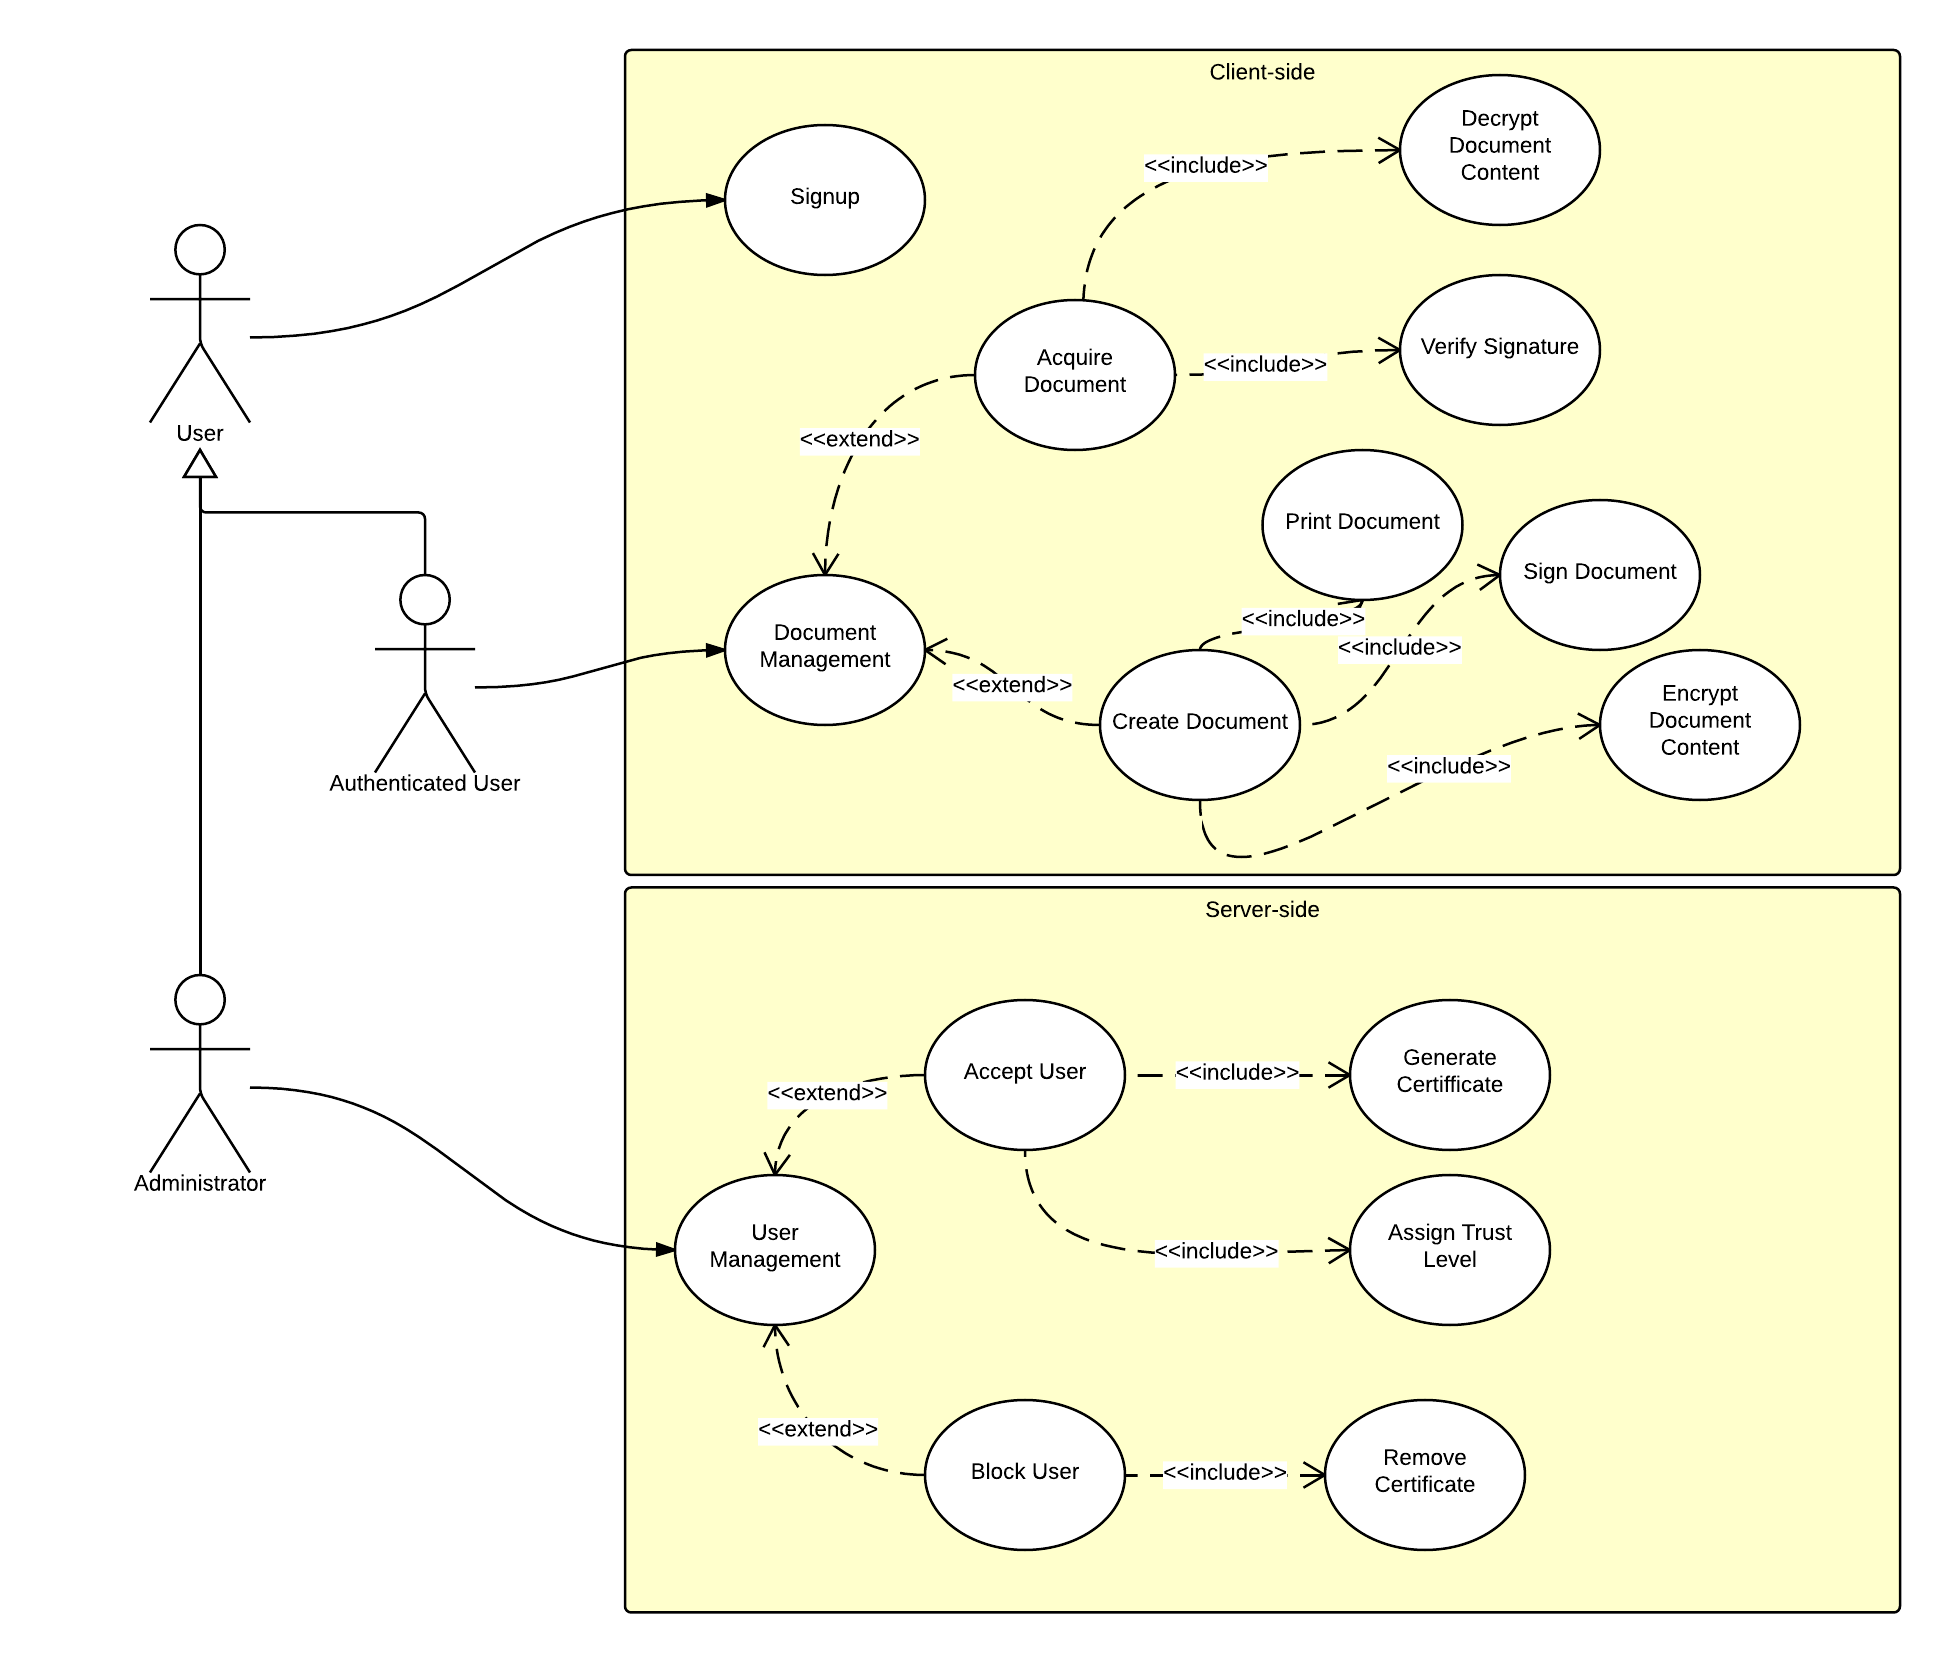
\includegraphics[scale=0.9]{Immagini/usecase}
		\caption[Use Case Diagram]{Diagramma dei casi d'uso del sistema software realizzato}
		\label{fig:usecase}
		\end{figure}
	\end{center}
La prima cosa che va evidenziata è che il tutto è strutturato secondo un architettura di tipo client/server. Questi due componenti dialogano tra di loro utilizzando una connessione sicura basata su SSL\footnote{Dettagli maggiori saranno dati nel paragrafo~\ref{sec:sicurezza}.}. Da quello che si può evincere, il server è un componente fondamentale che espone la funzionalità di \emph{provisioning} delle chiavi. Esso mantiene sia le chiavi di livello necessarie per la cifratura del documento, sia le chiavi pubbliche degli utenti registrati al sistema.

Da quello che si può vedere dalla figura~\ref{fig:usecase} nel sistema si hanno 3 attori importanti: l'amministratore, l'utente registrato (autenticato) e l'utente semplice che non ha mai utilizzato il sistema.
Come è stato già detto, l'amministratore si occupa di gestire l'accesso degli utenti. Questo vuol dire che ha piena facoltà di abilitare gli utenti all'utilizzo del sistema verificandone l'identità con procedure interne all'azienda che possono variare di caso in caso e che esulano completamente dagli scopi di questo progetto.
Oltre a questo può decidere di limitare l'accesso al sistema bloccando l'utente con una semplice procedura, grazie alla quale il server è in grado di comprendere se l'utente che si connette è autorizzato oppure no ad ottenere le chiavi di un certo livello.
Altro compito fondamentale è quello dell'assegnazione del Trust~Level che viene deciso in fase di abilitazione dell'utente al sistema. Tuttavia questo può essere anche cambiato successivamente. Grazie al Trust~Level, l'utente sarà abilitato a conoscere solo i segreti per cui è stato autorizzato, quindi l'assegnazione di questo parametro è fondamentale e richiede la massima attenzione.

L'utente registrato (o come riportato in figura~\ref{fig:usecase} ``autenticato'') rappresenta una qualsiasi persona che è stata abilitata dall'amministratore ad usare l'applicazione in tutte le sue funzionalità attuali. Un utente di questo tipo dispone di una coppia di chiavi asimmetriche RSA a $1024$ \texttt{bit} e di un certificato \texttt{X.509} che viene utilizzato per le connessioni al server che richiedono mutua autenticazione. L'utente autenticato ha la possibilità di comporre un documento, oscurarlo in alcune sue parti utilizzando le chiavi di livello a cui può accedere, e firmarlo con la propria chiave privata RSA. 
Naturalmente oltre alla composizione del documento, l'utente registrato ha anche la facoltà di leggere quello che è stato inviato a lui o agli utenti con il suo stesso Trust~Level\footnote{Si rimanda al paragrafo~\ref{sec:sicurezza} per una trattazione più approfondita di questo aspetto.}.

Per quanto riguarda l'utente semplice, si è sicuramente notato che questo ha l'unica facoltà di registrarsi al sistema. Questo perché non dispone ancora di un certificato da usare per l'autenticazione e quindi non ha alcuna possibilità di leggere le informazioni se non provando a fare un attacco sulla sicurezza del sistema o del documento cartaceo.

\section{Architettura}
	\label{sec:architettura}
Data una panoramica dei requisiti e delle funzionalità principali del sistema, si passerà adesso ad analizzare più in dettaglio l'architettura del sistema realizzato.
	\begin{center}	
		\begin{figure}[H]
		\centering
		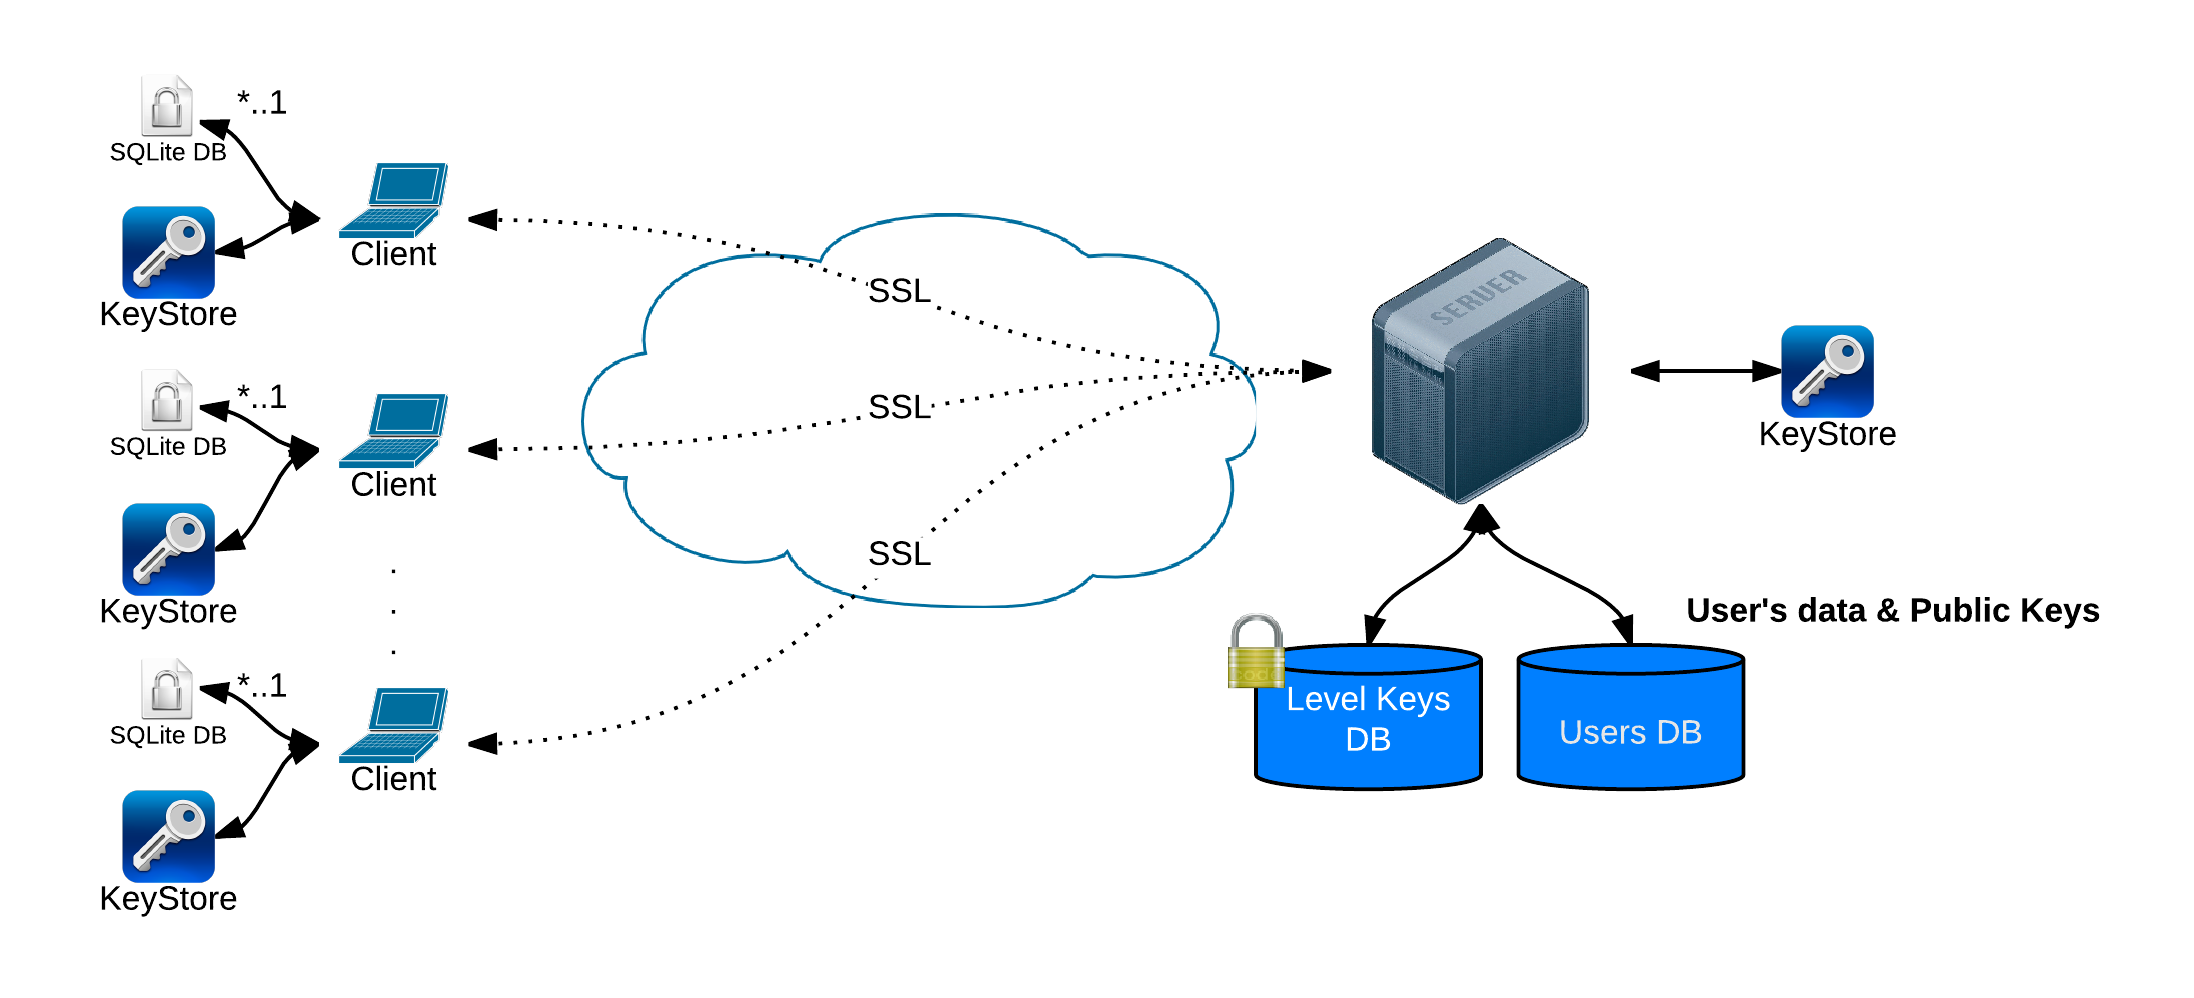
\includegraphics[scale=0.9]{Immagini/architettura}
		\caption[Architettura del sistema]{Questa figura rappresenta l'architettura del sistema software realizzato}
		\label{fig:usecase}
		\end{figure}
	\end{center}



\section{Gestione della sicurezza}
	\label{sec:sicurezza}
	%login - autenticazione forte
	%come si cripta: singolo/molti utenti
	%come si descripta
	%connessione al server
	%connessioni SSL - gestione certificati/keystore/mutua autenticazione	